\clearpage{\pagestyle{empty}\cleardoublepage}

\chapter{Sistemi di piggaggio delle condotte in pressione}\thispagestyle{empty} 
\chaptermark{Piggaggio}
Il piggaggio, o anche detto \textit{pigging}, è un'applicazione nella quale un dispositivo cilindrico o sferico chiamato scovolo (o \textit{pig}), opportunamente dimensionato, viene spinto all'interno di una condotta tramite variazioni indotte di pressione e flusso del mezzo presente all'interno, tramite l'introduzione di un mezzo esterno o tramite movimento meccanico al fine di pulire, ispezionare, dosare inibitori chimici lungo la tubazione oppure per isolare delle sezioni specifiche della rete.\\
L'origine del termine inglese \textit{pig} è tuttora incerto: se da una parte viene proposto come l'acronimo di \textit{Pipeline Intervention Gadget}, dall'altra si fa riferimento al rumore che provoca lo scorrimento dello scovolo in condotta, simile al verso di un maiale \parencite{varghese2011intelligent}.\\
Durante gli anni '40 negli Stati Uniti il piggaggio aveva come fine principale la rimozione di paraffina per migliorare l'efficienza delle condotte a olio, quindi per aumentare la produzione e sopperire all'alta domanda legata alle attività belliche della Seconda Guerra Mondiale.\\
Nel mondo oggi il piggaggio è impiegato per numerosi scopi e la strumentazione  è progettata dagli ingegneri in base alle necessità legate all'applicazione. 

\section{Configurazione degli scovoli}
L'assemblaggio e configurazione dello scovolo di servizio prevede numerose soluzioni:
\begin{itemize}
	\item \textbf{a mandrino} (\figref{fig:mandrel}): gli elementi dello scovolo sono assemblati sul corpo centrale tramite numerosi bulloni;
	\item \textbf{a bullone singolo} (\figref{fig:singlebolt}): simile allo scovolo a mandrino, gli accessori dello scovolo in questo caso sono inseriti tramite un'unica bullonatura longitudinale;
	\item \textbf{a telaio fisso} (\figref{fig:solidcast}): sia le tenute che gli elementi guida solo tenuti assieme da un singolo componente in poliuretano;
	\item \textbf{a schiuma} (\figref{fig:foampig}): solitamente con struttura aperta di poliuretano, questi scovoli sono disponibili a diversa densità, a seconda dell'applicazione richiesta. Il rivestimento aumenta la resistenza a usura e la stabilità dell'utensile;
	\item \textbf{sfere} (\figref{fig:spherepig}): possono essere piene o riempite con aria, acqua o glicol, possono essere usate come tamponi o rimozione liquidi;
	\item \textbf{articolato} (\figref{fig:articulated}): composto da due o più scovoli uniti tra loro con sistemi di accoppiamento universale. Rappresenta la configurazione base degli scovoli intelligenti;

\end{itemize}

\begin{figure}[htbp]
    \centering
    \subfloat[][A mandrino.]
    {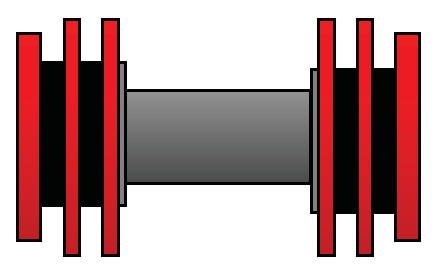
\includegraphics[height=.1\textheight]{fig/pig/configurazione/mandrel.eps}  \label{fig:mandrel}} \qquad
    \subfloat[][A bullone singolo.]
    {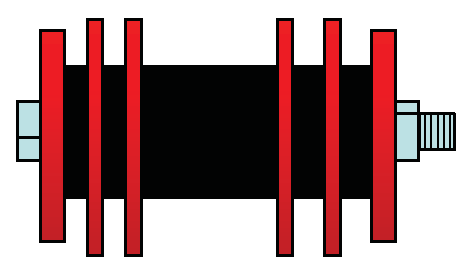
\includegraphics[height=.1\textheight]{fig/pig/configurazione/singlebolt.eps}  \label{fig:singlebolt}} \qquad 
    \subfloat[][A telaio fisso.]
    {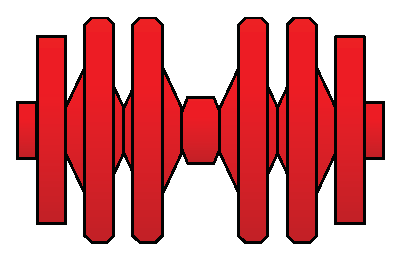
\includegraphics[height=.1\textheight]{fig/pig/configurazione/solidcast.eps}  \label{fig:solidcast}} \\
    \subfloat[][A schuma.]
    {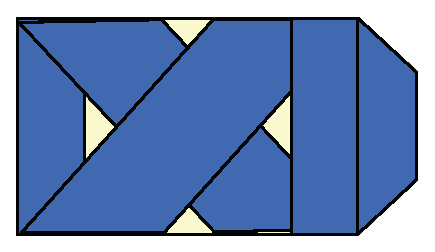
\includegraphics[height=.1\textheight]{fig/pig/configurazione/foam.eps}  \label{fig:foampig}} \qquad
    \subfloat[][Sfere.]
    {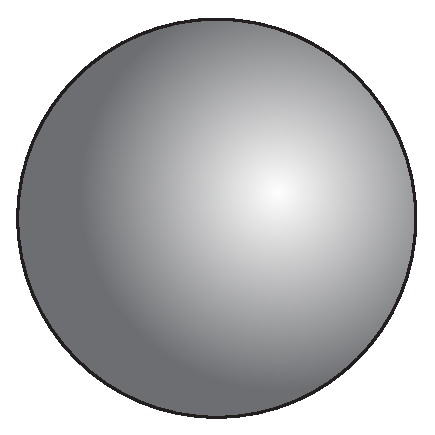
\includegraphics[height=.1\textheight]{fig/pig/configurazione/sphere.eps}  \label{fig:spherepig}} \\
    \subfloat[][Articolato.]
    {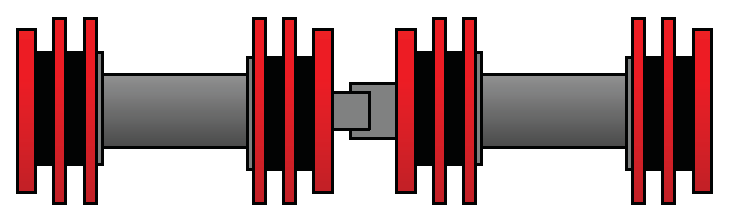
\includegraphics[height=.1\textheight]{fig/pig/configurazione/articulated.eps}  \label{fig:articulated}}
\caption{Configurazione dello scovolo \parencite{davidson2002introduction}.}
\label{fig:configurazione}
\end{figure}

Gli scovoli a mandrino e a bullone singolo si adattano alla richiesta specifica grazie all'installazione di diversi dispositivi sul corpo centrale:
\begin{itemize}
\item \textbf{spazzole} (\figref{fig:spazzole}):  impiegate in primo luogo per la rimozione di depositi compatti come calcare e prodotti da corrosione. Alcune spazzole sono specifiche per favorire l'azione degli inibitori di corrosione e dei biocidi in condotta;
\item \textbf{guarnizioni a tazza} (\figref{fig:tazze}): dispositivi di tenuta idraulica che consente lo spostamento unidirezionale dello scovolo attraverso la spinta di un fluido da monte. Sono utilizzati solitamente anche come dispositivi di \textit{batching};
\item \textbf{coppelle coniche} : molto simili alle guarnizioni a tazza, hanno una lieve variazione nella geometria della tenuta;
\item \textbf{dischi} (\figref{fig:dischi}): accessori utilizzati come tenute idrauliche, per la pulizia e come organi di supporto. A differenza delle guarnizioni a tazza e le coppelle coniche, uno scovolo dotato di dischi può muoversi in entrambe le direzioni;
\item \textbf{lame} (\figref{fig:lame}): tramite l'azione di taglio, provvedono alla rimozione di depositi morbidi come paraffina e fanghi, derivanti dal trasporto di olio in linea;
\item \textbf{magneti} (\figref{fig:magneti}): l'inserimento di potenti magneti sulla circonferenza permette allo scovolo non solo l'asportazione di materiale ferroso dalla condotta, ma anche di attivare i segnalatori posti all'esterno della condotta per monitorarne il tragitto;
\item \textbf{accessori per la misurazione}: possono essere di varia natura (calibri, dischi misuratori, dispositivi magnetici, etc.) e consentono l'ispezione interna della condotta.
%I singolo dispositivi possono essere accoppiati sullo stesso dispositivo, al fine di sopperire a più richieste con un unico passaggio dello scovolo in condotta (\figref{fig:assemblato}).
\end{itemize}

\begin{figure}[htbp]
    \centering
    \subfloat[][Scovolo con spazzole a molla.]
    {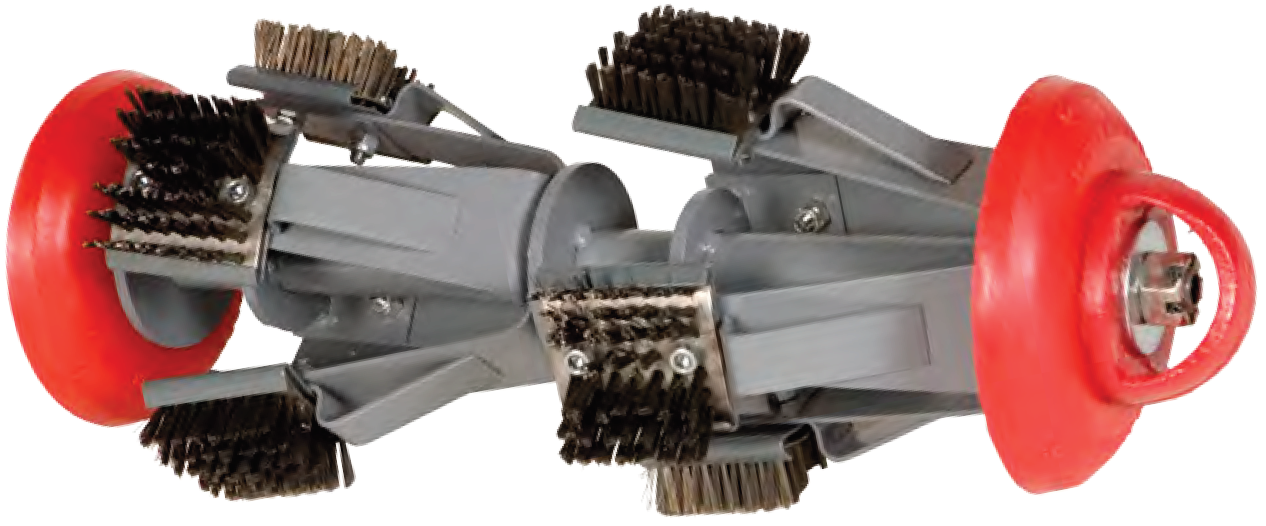
\includegraphics[height=.12\textheight]{fig/pig/tool/spazzolemolla}  \label{fig:spazzole}} \qquad
    \subfloat[][Scovolo con guarnizioni a tazza.]
    {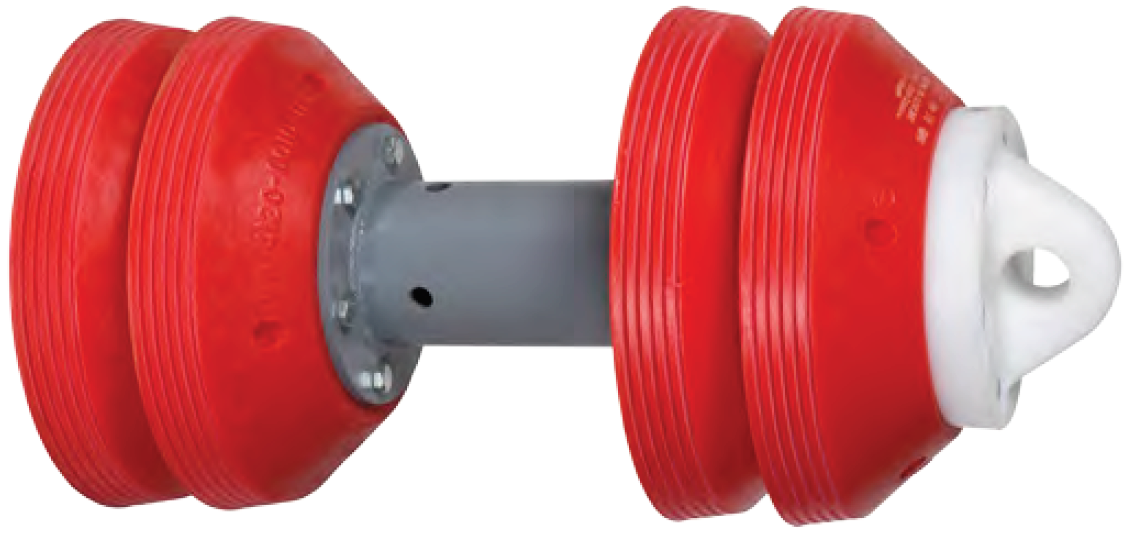
\includegraphics[height=.12\textheight]{fig/pig/tool/tazze}  \label{fig:tazze}} \qquad
    \subfloat[][Scovolo con dischi.]
    {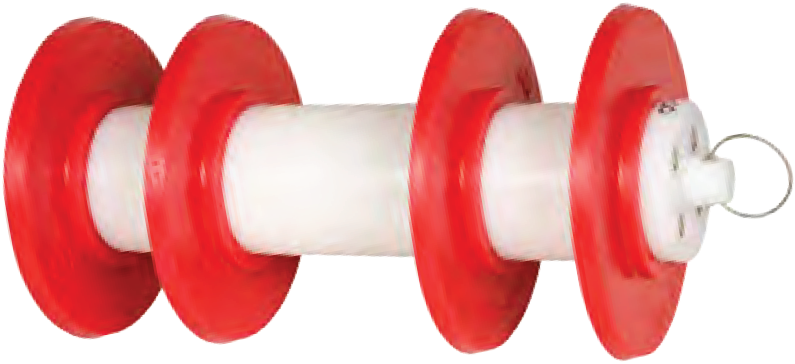
\includegraphics[height=.12\textheight]{fig/pig/tool/dischi}  \label{fig:dischi}} \\
    \subfloat[][Scovolo con lame di poliuretano.]
    {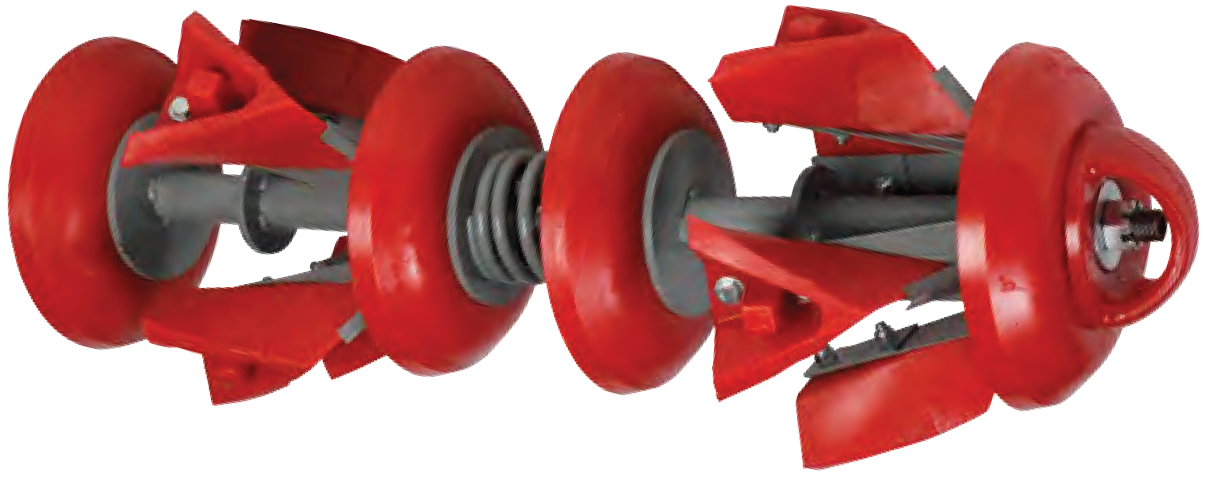
\includegraphics[height=.12\textheight]{fig/pig/tool/lame}  \label{fig:lame}} \qquad
    \subfloat[][Scovolo con magneti sulla circonferenza.]
    {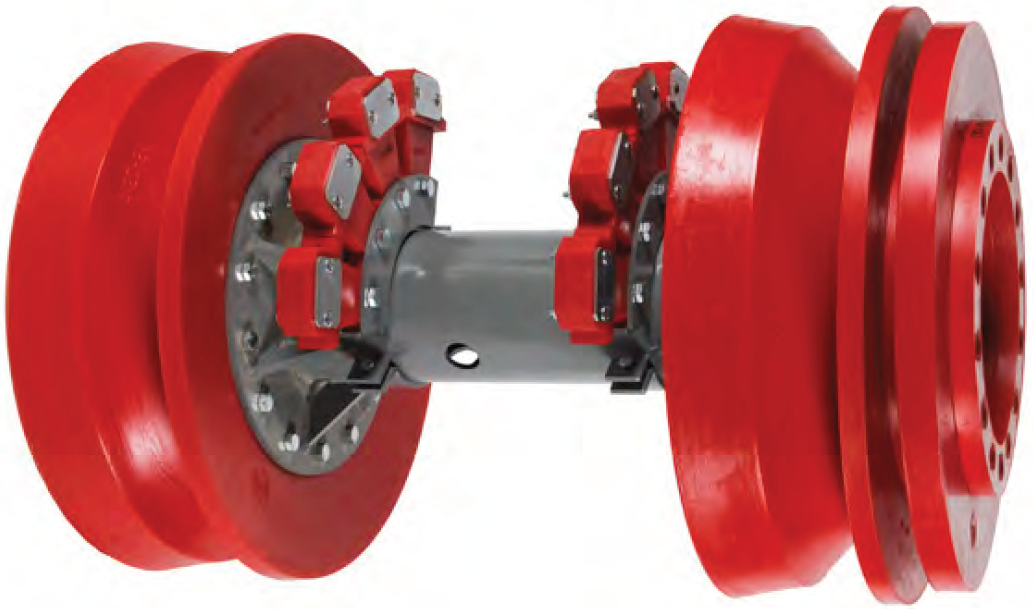
\includegraphics[height=.12\textheight]{fig/pig/tool/magneti}  \label{fig:magneti}} \qquad
%    \subfloat[][Scovolo con spazzole circolari, guarnizioni a tazza e dischi.]
%    {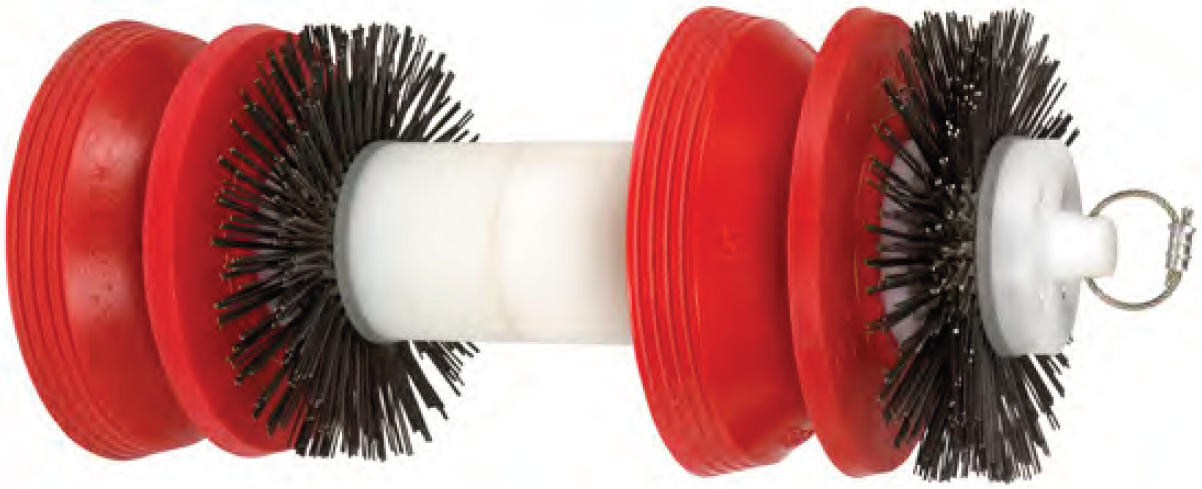
\includegraphics[height=.12\textheight]{fig/pig/tool/assemblato}  \label{fig:assemblato}}
\caption{Componenti tipici di uno scovolo di servizio \parencite{williamson2015guide}.}
\label{fig:configurazione}
\end{figure}

\section{Obiettivi del piggaggio}
Il piggaggio di una condotta viene oggi eseguito in tutte le fasi di vita di un impianto di processo. Data la sua versatilità, è di consuetudine per tutti i settori dell'industria di processo, perciò non esistono delle classificazioni universali degli scovoli impiegati. Una generica distinzione tra \textit{pig} può essere fatta in base all'operazione richiesta: si parla quindi di scovoli di servizio, scovoli per l'ispezione interna e scovoli gel.

\subsection{Scovoli di servizio}
Qui di seguito sono elencati i motivi legati generalmente all'impiego di scovoli di servizio:
\begin{itemize}
	\item \textbf{pulizia della condotta}: utile per migliorare le condizioni di flusso;
	\item \textbf{separazione dei fluidi} o \textit{\textbf{batching}}: scovoli di separazione tra diversi prodotti chimici da applicare in condotta;
%		\item \textbf{ispezione interna}: è importante monitorare le condizioni interne della condotta, così da prevedere eventuali rotture o imprevisti di produzione. Gli scovoli possono assumere numerose configurazioni (forma e dimensioni), obiettivo ultimo è il rilevamento di ammaccature, consumo interno della parete interna e crepe.
	\item \textbf{spiazzamento della condotta}: specialmente nelle condotte a gas, gli scovoli possono essere utilizzati per spiazzare delle formazioni liquide indesiderate in condotta.
\end{itemize}

\subsubsection{Pulizia}
Gli scovoli pulenti sono impiegati per mantenere dei livelli di efficienza minimi in condotta. Nel settore degli idrocarburi, qualunque riduzione di portata corrisponde a un mancato introito giornaliero. La riduzione della portata è legata all'attrito e a fattori fisici. Nelle condotte a gas i problemi di produzione sono legati alla presenza di elementi corrosivi, detriti e depositi, polveri e condensati. Nel caso del greggio le condotte risentono della presenza di sabbia e paraffina adesa alle pareti interna della tubazione.\\
Si valuta l'efficienza di una condotta tramite considerazioni tecniche su flusso, cadute di pressione e costi operativi. Nel momento in cui la condotta necessità di una pulizia interna, si inserisce uno scovolo  lungo il tratto interessato.\\
\begin{figure}[htbp]
	\centering
	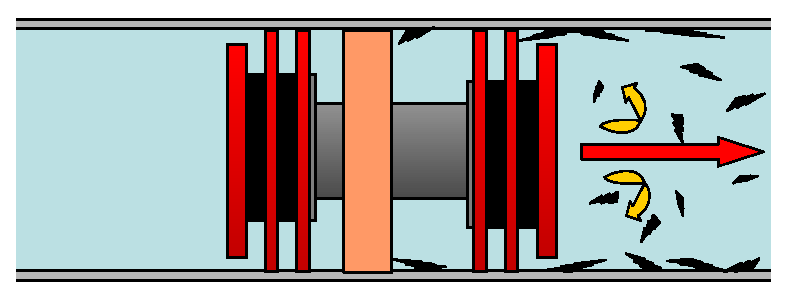
\includegraphics[width=.7\textwidth]{fig/pig/cleaning.eps}
	\label{fig:cleaningpig}
	\caption{Scorrimento dello scovolo di pulizia in condotta e rimozione dei depositi solidi in condotta \parencite{davidson2002introduction}.}
\end{figure}
La configurazione migliore del \textit{pig} pulente consiste in dischi, guarnizioni a tazza e spazzole radiali a molla o lame in poliuretano. I dischi consentono di spingere via i residui solidi oltre a fornire un buon supporto, le guarnizioni provvedono alla tenuta, le spazzole consentono la rimozione di ruggine, detriti e altri residui solidi mentre le lame sono impiegate in condotte a olio, grazie alla maggiore efficacia sulla paraffina e la facilità di pulizia al termine dell'applicazione. Nella pulizia di condotte con mezzi liquidi gli scovoli possono essere dotati di \textit{bypass}, ugelli longitudinali che convogliano del liquido in pressione da monte a valle, evitando così il deposito dei solidi sul fondo e riducendo la velocità di scorrimento del dispositivo.


\subsubsection{Spiazzamento}
Per spiazzamento della condotta si intende la completa sostituzione di un mezzo fluido con un altro. Gli scovoli di spiazzamento o separazione, tramite meccanismi di spinta e di tenuta, consentono di effettuare queste operazioni. Numerose sono le operazioni che necessitano l'impiego di questi dispositivi.\\
I test di tenuta idraulica di una condotta prevedono lo spurgo totale, il riempimento con acqua e la pressurizzazione della linea per un determinato periodo di tempo tramite scovoli di spiazzamento. Altri impieghi sono la separazione tra idrocarburi e gas inerte per poter effettuare riparazioni sul campo o lo spiazzamento di liquidi indesiderati da linee a gas.\\
La configurazione generica è rappresentata dagli scovoli a quattro tazze di tenuta, tenute in contatto con le pareti della condotta. Per ovviare alle variazioni di diametro interno, si utilizzano delle guarnizioni a tazza a più labbra di tenuta (\textit{multi-lipped cup}).\\
Alcuni scovoli a schiuma consentono dei buoni livelli di tenuta idraulica per distanze medio-brevi con una spesa relativamente bassa.\\
Gli scovoli a dischi bidirezionali sono tipicamente usati nelle operazioni di riempimento e spiazzamento acqua in condotta, associati quindi ai test di tenuta. La possibilità di agire in direzione doppia consentono la ricollocazione del dispositivo in posizione iniziale nel caso in cui si preveda la possibilità di blocco in condotta.\\
Le sfere sono la soluzione ideale per la rimozione di liquidi da linee a gas. I sistemi di piggaggio a sfere sono progettati per il lancio e la ricezione in automatico, con un numero di sfere che può variare in base alle richieste specifiche. Sul punto di ricezione, si prevede l'installazione di uno \textit{slug catcher} per ovviare al volume di liquido associato alle sfere. Le condotte a gas sono normalmente progettate per l'uso di sfere, ciò non vuol dire che possano essere piggabili da scovoli convenzionali.\\
Schiume a bassa densità sono impiegate per asciugare la condotta dopo l'operazione di spiazzamento d'acqua. Questi \textit{pig} hanno come unico svantaggio la possibilità di potersi bloccare in opera.\\
 
\subsubsection{Separazione dei fluidi}
In alcune applicazioni si richiede l'immissione di uno o più prodotti separatamente. Nella condotta si possono creare delle condizioni di "contaminazione" a causa di:
\begin{itemize}
	\item regime di flusso;
	\item geometria della condotta;
	\item procedure operative.
\end{itemize}
Al fine di ovviare al contatto tra i diversi prodotti, si impiegano in condotta degli scovoli tampone o \textit{batching pig}, dispositivi di tenuta idraulica in grado di evitare il contatto tra i singoli \textit{slug}. La \figref{fig:batching} mostra un'applicazione tipica: i primi due \textit{slug} di acqua dolce provvedono alla desalinazione precedentemente percorsa da acqua di mare, mentre gli \textit{slug} di glicol permettono la deidratazione e l'inibizione degli idrati.

\begin{figure}[htbp]
	\centering
	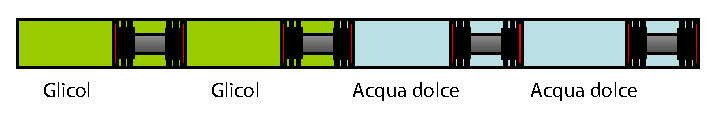
\includegraphics[width=\textwidth]{fig/pig/batching.eps}
	\label{fig:batching}
	\caption{Desalinizzazione della condotta con treni di acqua dolce, glicol e azoto in successione \parencite{davidson2002introduction}.}
\end{figure}

Gli scovoli impiegati per la separazione di prodotti sono gli stessi per lo spiazzamento: in particolar modo si parla di guarnizioni a tazza, coppelle coniche e dischi bidirezionali.

\subsection{Strumenti di ispezione interna}
Questi dispositivi provvedono a fornire informazioni sulle condizioni della condotta, così come l'estensione e la localizzazione di qualsiasi problema presente. Gli scovoli di ispezione interna più semplice sono di misurazione meccanica.\\
Lo scovolo a piastra spessimetrica (\figref{fig:gauging}) è un dispositivo di misurazione molto semplice: lo strumento di misura consiste in un disco dal diametro pari al 95\% di quello della condotta interna. Associato a un emettitore acustico, lo scovolo emette un segnale quando si presenta un restringimento, fornendo quindi indicazioni agli operatori per la riparazione della condotta. \\
Lo scovolo calibro (\figref{fig:caliper}) è utile alla misurazione della geometria interna della condotta. Un sistema di leve metalliche radiali, in questo caso definito calibro, è collegato a un dispositivo di registrazione interno, il quale tiene traccia del profilo interno della condotta in funzione della posizione. 

\begin{figure}[htbp]
    \centering
    \subfloat[][Scovolo a piastra spessimetrica.]
    {\makebox[0.3\textwidth]{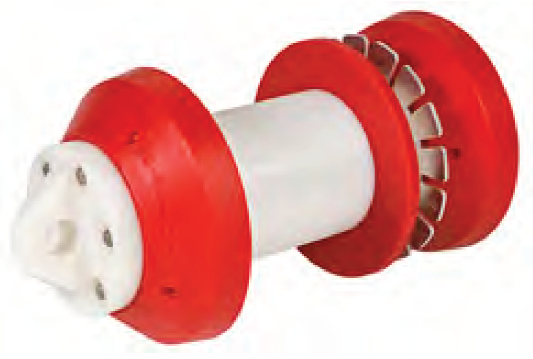
\includegraphics[height=.12\textheight]{fig/pig/gauging}}  \label{fig:gauging}} \qquad
    \subfloat[][Scovolo calibro.]
    {\makebox[0.3\textwidth]{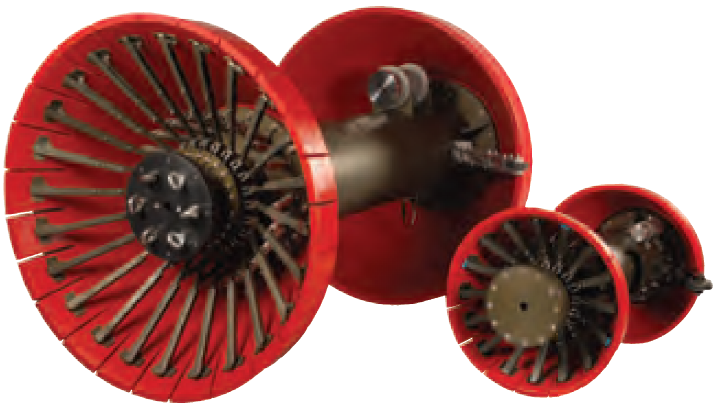
\includegraphics[height=.12\textheight]{fig/pig/caliper}}  \label{fig:caliper}}
\caption{Scovoli di ispezione interna tradizionali \parencite{williamson2015guide}.}
\label{fig:internalinspection}
\end{figure}

Al fine di venire incontro alle esigenze di misurazione sempre più precise, negli ultimi anni sono state sviluppate delle tecnologie che non impiegano dispositivi meccanici per l'ispezione: sono definiti scovoli intelligenti o \textit{smart pig}.

\subsubsection*{Scovoli intelligenti o \textit{smart pig}}
Questi scovoli sono strumenti utili all'ispezione della condotta, capaci di svolgere operazioni complesse come mappatura, misurazioni geometriche, individuazione di crepe, assottigliamento localizzato della condotta. Oggi il piggaggio intelligente è considerato un settore industriale indipendente, data l'importanza dell'applicazione.\\
Il concetto di piggaggio intelligente nasce nel 1963 dal settore ricerca della Shell e brevettarono un metodo di ispezione basato sulle correnti parassite.\\
Attualmente le due tecnologie maggiormente impiegate sono gli scovoli a dispersione di flusso magnetico (\textit{Magnetic Flux Leakage}, MFL) e gli scovoli a ultrasuoni.
Gli scovoli MFL (\figref{fig:smartpig}) si basano sul principio della misurazione della dispersione di flusso magnetico legata al volume delle perdite metalliche, quindi allo spessore della parete della condotta. Questo scovolo funziona in mezzi gassosi e/o liquidi. La valutazione finale dei dati viene raffinata negli anni poiché è frutto di misurazioni indirette, legate quindi a un processo interpretativo.\\
L'alternativa all'MFL consiste nell'impiego di misure a ultrasuoni. In questo caso la parete della condotta viene calcolata tramite misurazione diretta, il ché rende questa tecnologia molto più affidabile rispetto al controllo della dispersione di flusso magnetico. Ha lo svantaggio di non potere essere utilizzata con mezzo gassoso: il suo impiego in questo caso prevede l'utilizzo di un mezzo liquido di riempimento prima di poter effettuare le operazioni di misura.

\begin{figure}[htbp]
	\centering
	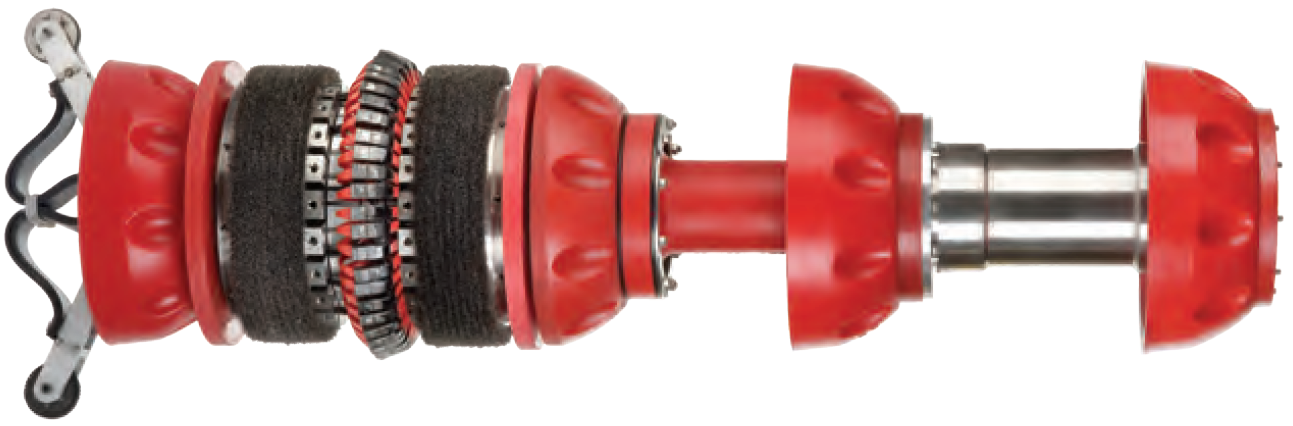
\includegraphics[width=.6\textwidth]{fig/pig/smartpig}
	\label{fig:smartpig}
	\caption{Scovolo a dispersione di flusso magnetico \parencite{williamson2015guide}.}
\end{figure}

La ricerca nel settore degli scovoli intelligenti è molto attiva e le soluzioni in commercio sono innumerevoli. Fra queste troviamo i \textit{pig} a neutroni, utili per rilevare nelle condotte sottomarine le sezioni non più sotterrate (\textit{span}). Le aree a contatto con l'acqua sono soggette a maggiori fenomeni di danneggiamento. Nella pratica comune vengono impiegati degli strumenti esterni per rilevare degli \textit{span}, attraverso lo scovolo a neutroni si riducono il numero di indagini e si migliora l'accuratezza dell'analisi.\\
Altri esempi includono delle videocamere montate sullo scovolo, impiegate per l'ispezione interna visuale oppure scovoli per il rilevamento di curvature in condotte nelle aree artiche, corrispondenti a sollecitazioni locali causate dalle differenze di temperatura.

\subsection{Scovoli gel}
In questo caso non si parla di dispositivi di forma propria, bensì di sistemi a base di liquidi gelificati che sono sviluppati per le operazioni ausiliare in condotta come avvio della produzione, operazioni di supporto agli scovoli tradizionali o programmi di mantenimento.\\
La maggior parte dei gel impiegati sono a base acqua, tuttavia possono essere anche a base di glicol, metanolo o altre sostanze liquida a seconda delle esigenze tecniche.\\
I tipi di scovoli gel disponibili sono:
\begin{itemize}
	\item \textbf{gel di \textit{batching}};
	\item \textbf{gel per cattura di detriti};
	\item \textbf{idrocarburi gelificati};
	\item \textbf{gel disisdratanti}
\end{itemize}

I principi applicativi degli scovoli gel vanno dalla separazioni delle diverse fasi liquide alla rimozione dei detriti, dai test di riempimento condotta allo spiazzamento dei liquidi indesiderati, fino all'impiego di sostanze chimiche come inibitori o biocidi. Importante sottolineare l'impiego del gel nello sblocco di scovoli tradizionali incastrati in condotta.

\begin{figure}[htbp]
	\centering
	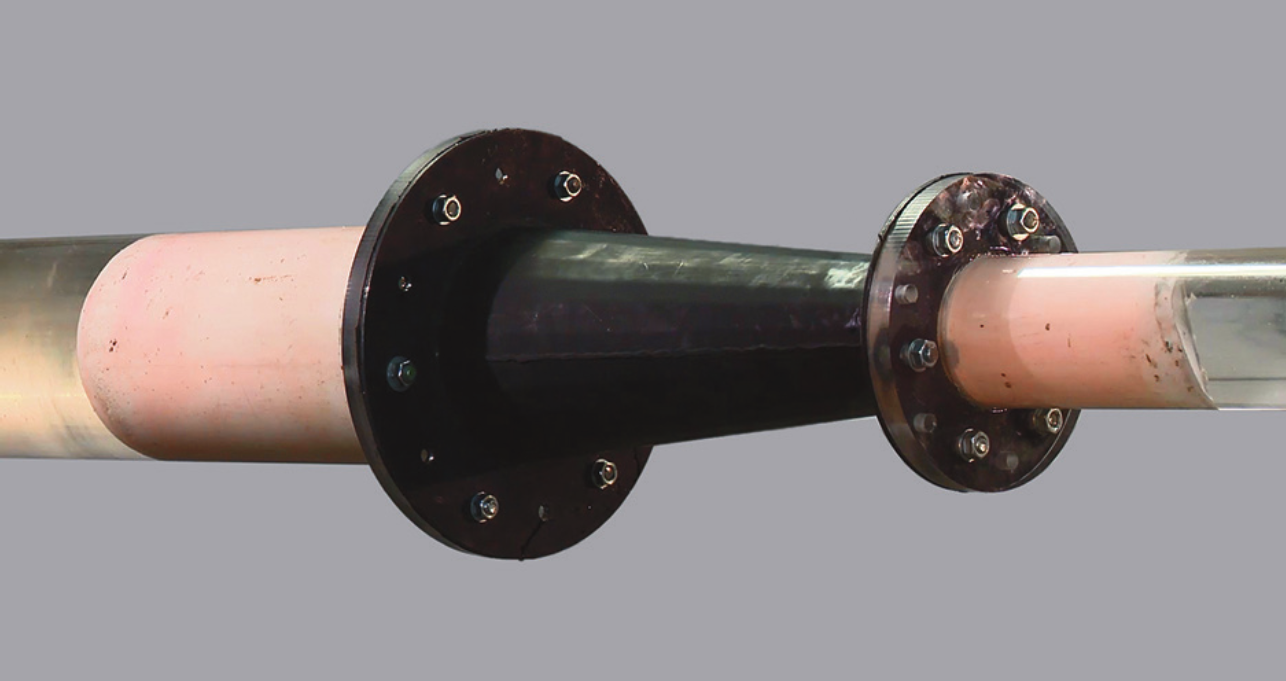
\includegraphics[width=\textwidth]{fig/pig/gelpig}
	\label{fig:gelpig}
	\caption{Scovolo gel EVO-Pig, Aubin Ltd \parencite{johnston2015breaking}.}
\end{figure}


%-------------------------------------------------------------------

\section{Progettazione del sistema di condotte per il piggaggio}
Il sistema deve essere progettato in modo tale da evitare imprevisti nelle operazioni di piggaggio. Di conseguenza ci sono degli importanti elementi di design da tenere in considerazione.
\subsection{Lunghezza del cammino del pig}
\subsection{Raggio di curvatura}
\subsection{Tipologia di valvole presenti}
\subsection{Indicatori di passaggio del pig}
\subsection{Raccordi}
\subsection{Condotte laterali}
\subsection{Raggio interno di condotta}
\subsection{Condotte a doppio diametro}


\section{Procedure di lancio e recupero del pig}

\subsection{Condotte a liquido}
\subsubsection{Procedure di lancio pig per condotte a liquido}
\subsubsection{Procedure di recupero pig per condotte a liquido}

\subsection{Condotte a gas}
\subsubsection{Procedure di lancio pig per condotte a gas}
\subsubsection{Procedure di recupero pig per condotte a gas}

\subsection{Esempi di configurazione di sistemi di piggaggio}
\subsubsection{Lancio verticale}
\subsubsection{Lancio standard del pig}
\subsubsection{Lancio doppio o duale}
\subsubsection{Sistema di batch automatico}
\subsubsection{Lancio inclinato}
\subsubsection{Lancio combinato pig/sfera}
\subsubsection{Sistemi di piggaggio automatico}
\subsubsection{Lancio del pig di ispezione in linea}

\section{Piggaggio di una condotta onstream con mezzo gassoso o idrocarburi raffinati}
\subsection{Scelta del pig}
\subsection{Velocià}
\subsection{Frequenza}
\subsection{Prestazioni}

\section{Bloccaggio del pig o "stuck pig"}
\subsection{Soluzioni}
\subsection{Fasi operative}
\subsection{Sviluppo futuro}